\chapter{Architecture Constraints}

\section{Environment}
\label{sec:Environment}
In the context of an AUTOSAR ECU, RTA-SUM modules are technically built as Application Software Components. Therefore, each RTA-SUM module requires a full AUTOSAR SW stack to run. We assume that the following AUTOSAR SW will be used:
\input{generated/tables/tools.tex}

\section{Layers Definition}
The SUM\_SSFM is a software module in the application layer of the standardized architecture of AUTOSAR (Figure~\ref{fig:Layers}). 
It interacts with other RTA-SUM modules and components of the BSW. In the latter case, the RTE is the means through which the interaction takes place.
\begin{figure}[htp]
\centering
	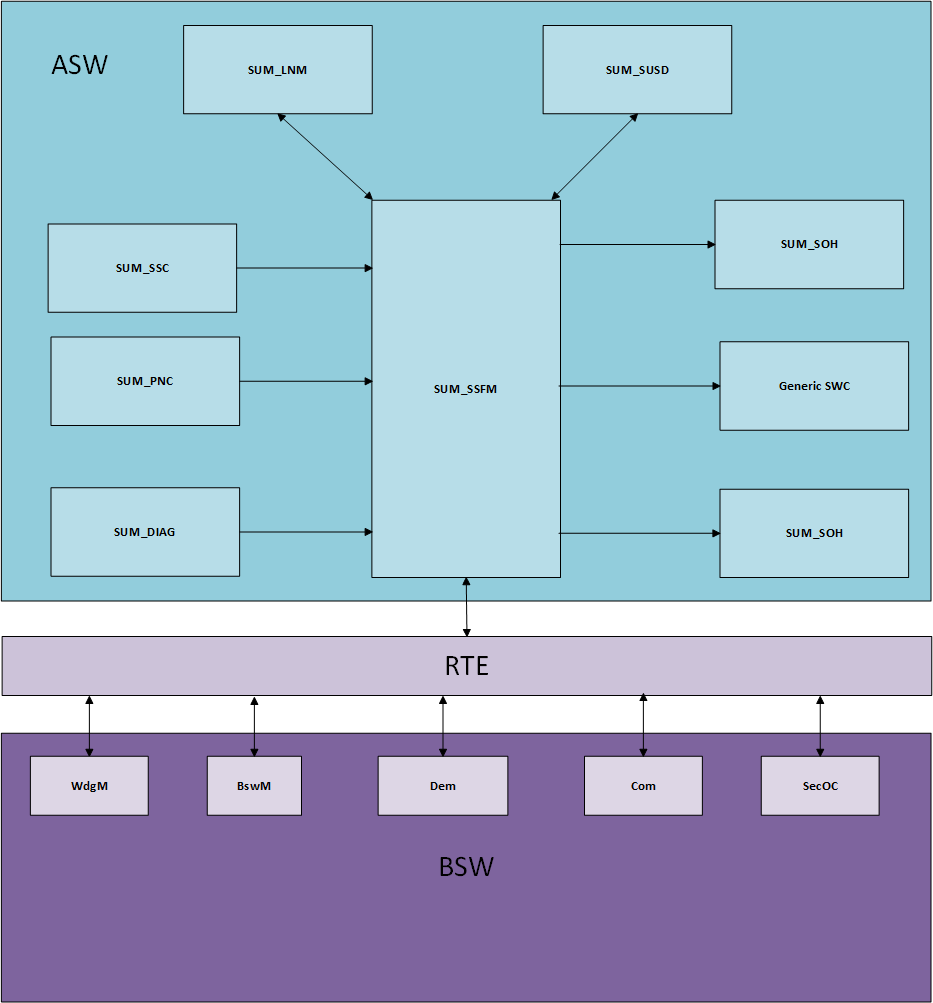
\includegraphics[scale=0.5]{images/SSFM_System_Block_View.png}
	\caption{System layer overview.}
	\label{fig:Layers}
\end{figure}

\section{Generic component interface}

The external interfaces of RTA-SUM module, and most of the interactions among SUM modules are specified in GM SDV-8002.

Section \ref{sec:portInterfaces} reports all interfaces that are implemented on RTA-SUM SSFM ports to the RTE.

\section{Other constraints and assumptions}

SSM has service needs that are provided by the AUTOSAR BSW. For an ECU to implement SSM, the following must be true:
\begin{itemize}
\item The ECU must have an RTE that supports:
	\begin{itemize}
	\item Sender / Receiver and Client /Serverport interface
	\item Callbacks from the comm stack BSW for
		\begin{itemize}
		\item Deadline monitoring ComTimeoutNotification: Com\_CbkRxTOut callback function
		\item Message received notification: Com\_CbkRxAck()
		\end{itemize}
	\item Invalid Value signal reception: Rte\_COMCbkInv\_<sn> (for signals and group signals)
	\end{itemize}
\item The ECU must have AUTOSAR SecOC module
\item The ECU must have AUTOSAR E2E library
\item The ECU must have AUTOSAR E2E transformer
\item The ECU must have AUTOSAR BSW Mode Manage module.
\item The ECU must have AUTOSAR COM Manage module..
\item The ECU must have AUTOSAR COM Module.
\item The ECU must have AUTOSAR NvM Module.
\item The ECU must have AUTOSAR LIN State Manager module.
\item The ECU must have AUTOSAR LIN Interface module.
\item The ECU must have interface to following SUMs: SUM\_PNC, SUM\_TCS, SUM\_SOH.
\end{itemize}

ERRH has service needs that are provided by the AUTOSAR BSW. In order for an ECU to implement ERRH, the following must be true:
\begin{itemize}
\item The ECU must have an RTE that supports:
	\begin{itemize}
	\item Client / Server port interface
	\item Sender / Receiver port interface
	\end{itemize}
\item The ECU must have BSW that fulfills the requirements of AUTOSAR Diagnostic Event Manager module.
\item It is assumed that the ECU initialization sequence is designed such that any NVM needed for the ERRH function is available prior to ERRH being initialized.
\end{itemize}

